\section{Evaluation}
\label{sec:evaluation}




We implement our concurrent sketches and evaluate its
performance.
Our implementation for both concurrent sketches is based on the
algorithms implemented in DataSketches~\cite{}, which is a Java
open source library of stochastic streaming algorithms.
%We implemented our both concurrent sketches inside
%DataSketches~\cite{}, which is a Java open source library
%of stochastic streaming algorithms.
In both cases (quantiles and theta), we build our concurrent
sketch on top of the sequential sketch implementation, which was
already very optimized in the library.

In Section~\ref{sub:imp} we give some of the implementation
details.
In Section~\ref{sub:setup} we describe the experiment setup.
In Section~\ref{sub:thetaExp} we compare our Concurrent Theta
sketch with the sequential implementation given in
DataSketches library, and in Section~\ref{sub:quantilesExp} we do
it for the quantiles sketch. 


\subsection{Implementation}
\label{sub:imp}

To avoid false sharing, unnecessary cash misses, and memory
flashes we let each worker thread to locally maintain its private
part of the sketch.
One way to achieve this is by using thread local memory.
However, since a single sketch update requires so little
computations, we measure that accessing thread local memory per
every operation decreases the update throughput by 30 percent.
Therefore, we choose a different approach that requires little
changes in the API.
Given a shared sketch, instead of calling its methods
directly, every worker thread first wraps it with a context
(sometime called handler) that implements the same interface as
the sketch, and then access the sketch only through its context.
The context is stored the memory that is close to the core
the thread runs on, and it has all the necessary information
(e.g., thread id) that the worker thread has to know in order to 
work with the shared sketch.

  

\subsection{Experiment Setup}
\label{sub:setup}

The experiments were run on a dedicated machine with four Intel
Xeon E5-4650 processors, each with $8$ cores, for a total of
$32$ threads (with hyper-threading disabled).
For the experiments we use microbenchmarks, and consider two
representative workloads: (1) an \emph{update-only} workload in
which a sketch is built from a stream, and (2) a \emph{mixed}
workload in which there is a single reader that continuously read
from the sketch, while the other threads build it.
We run every experiment for 30 seconds. 
Our baselines are the the sketches' sequential implementations
given in the DataSketches library that we wraped with a read/write lock
to allow concurrency.

\subsection{Theta sketch}
\label{sub:thetaExp}

Since we are not familiar with prior works on concurrent Theta
and quantiles sketches, our only baseline is the very optimized
sequential implementation given in DataSketches that we wrap with
a read/write lock.
As we mention before, the cost of acquiring a lock in every
operation on the sketch is very high since the sketches are
inherently very fast data structures.
Figure~\ref{fig:LockIsBadTheta} compares the throughput of the
sequential implementation Theta sketch given in DataSketch with
ans without a lock.

\begin{figure}[t!]
    \centering
    \begin{subfigure}[t]{0.49\textwidth}
        \centering
        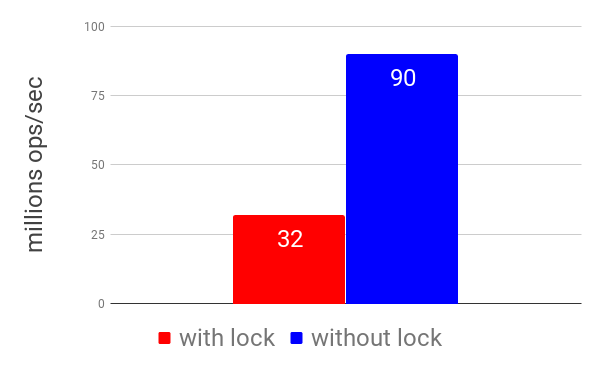
\includegraphics[width=3.2in]{images/seqTheta}
        \caption{}
        \label{fig:LockIsBadTheta}
    \end{subfigure}%
    ~ 
    \begin{subfigure}[t]{0.49\textwidth}
        \centering
        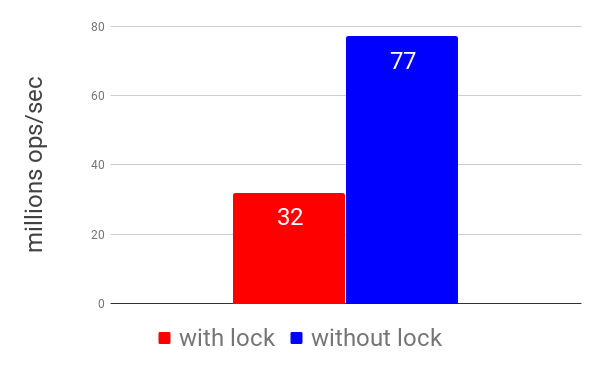
\includegraphics[width=3.2in]{images/seqQuantiles}
        \caption{}
        \label{fig:LockIsBadQuantiles}
    \end{subfigure}
    \caption{}
    \label{fig:sequntial}
\end{figure}

In Figure~\ref{fig:ConccurentTheta} we compare the scalability
between our concurrent sketch and the original sketch wrapped
with a read/write lock in a update only workload.
As expected, the lock based sequential sketch does not scale, and
in fact it performs worse when accessed concurrently by many
threads.
However, our sketch achieves almost perfect scalability.
In this graph we show results with the following parameters:
Every local buffer contains 16 items, while the size of the
shared sketch is 4096 items.
We run each experiment for 30 seconds.
It is important to note the we also tried smaller local buffers,
and shorter runs and the results were the same.

\begin{figure}[h]
  \centering
  \includegraphics*[width=4in]{images/concurrentThetaGraph}
  \caption{}
   \label{fig:ConccurentTheta}
\end{figure}




In Figure~\ref{fig:ConccurentThetaReads} we compare the
throughput of the reader, between
our concurrent sketch and the original sketch wrapped with a
read/write lock, in a mix workload.
We also measured the updates throughput in the present of one
reader, but we omit this graph since it looks exactly the same as
the one in Figure~\ref{fig:ConccurentTheta}.
We can see that in our sketch the reader is able to read 380
millions time in a second independtly of the number of concurrent
writers, while sequential lock-based's sketch is able to support
only 0.2 millions per second in case of one conccurent writer,
and it goes down to 0.0006 millions reads per seocnd when the
number of writers grows to 28.
We achieve stable very high throughput because the reader in our
sketch simply read one atomic variable, which does not
interfere the background thread, while in the sequential
lock-based's sketch the reader pay the fence price in addition
to competing with all the writers on acquiring the lock.  



\begin{figure}[h]
  \centering
  \includegraphics*[width=4in]{images/concurrentThetaReads}
  \caption{}
   \label{fig:ConccurentThetaReads}
\end{figure}




\subsection{Quantiles sketch}
\label{sub:quantilesExp}

As for the Theta sketch, our only baseline here is a very
optimized sequential implementation given in the DataSketch
library.
Figure~\ref{fig:LockIsBadQuantiles} shows that as in the Theta
case, wrapping the sequential quantiles sketch with a read/write
lock decreases throughput by almost a factor of 3 even with a
single thread.

In Figure~\ref{fig:ConccurentQuantilesUpdate} we compare the
throughput of our Quantiles sketch to the baseline.
First, note that the baseline does not scale, and moreover, it
achieves best result with a single worker thread.
Our sketch, on the contrary, scale perfectly when every thread
has enough local levels.
It clearly follows from the graph that in order for the
background thread to support more worker threads we have to
increase the number local levels.
O local levels are enough for 2 threads, 2 local levels are good
for 12 threads, and for perfect scalability on our machine in
update-only workload we need 4 local levels.


%we can shoe also the partition result and talk about locality.
% 1. the prcie of fences
% 2. the price of bringing new sketche to local memory and pay
% the cash missess.

\begin{figure}[h]
  \centering
  \includegraphics*[width=4in]{images/QuantilesUpdate}
  \caption{}
   \label{fig:ConccurentQuantilesUpdate}
\end{figure}

In Figure~\ref{fig:ConccurentQuantilesReader} we consider a
mixed workload to check how a single reader impact the update
throughput.
Since the reader in this case continuously reads the atomic
bitPattern variable, and thus forces the background thread to
flash its local memory more often, we see that the background
thread indeed works harder.
Instead of 4 levels in the update-only workload, we now need 5
local levels for perfect scalability, and we can also see that
0 and 2 local levels allow the background thread to support less
worker threads than in the update-only workload.




\begin{figure}[h]
  \centering
  \includegraphics*[width=4in]{images/QuantilesMixed}
  \caption{}
   \label{fig:ConccurentQuantilesReader}
\end{figure}

